\chapter{Images in Testing Set}
\label{app:01}
This appendice are show the for testing sets for table \ref{tab:data-motor} and table \ref{tab:data-car}
\begin{center}
    \begin{figure}[H]
        \centering
      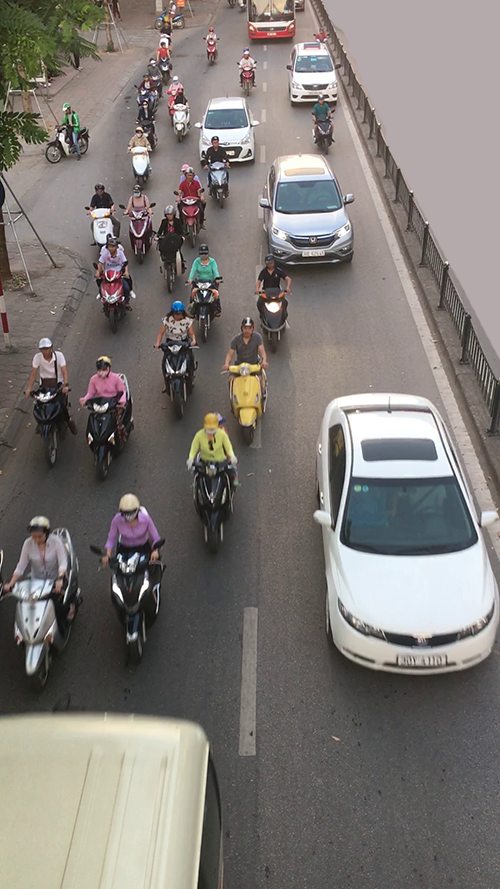
\includegraphics[width=0.5\textwidth]{Chapters/Fig/07}
      \caption{Image 7}
      \label{fig:img07}
  \end{figure}
\end{center}

\begin{center}
    \begin{figure}[H]
        \centering
      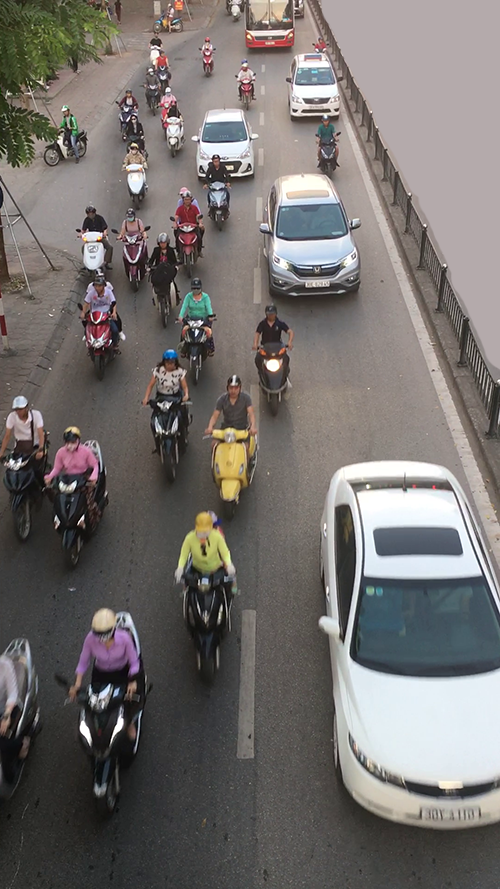
\includegraphics[width=0.7\textwidth]{Chapters/Fig/08}
      \caption{Image 8}
      \label{fig:img08}
  \end{figure}
\end{center}

\begin{center}
    \begin{figure}[H]
        \centering
      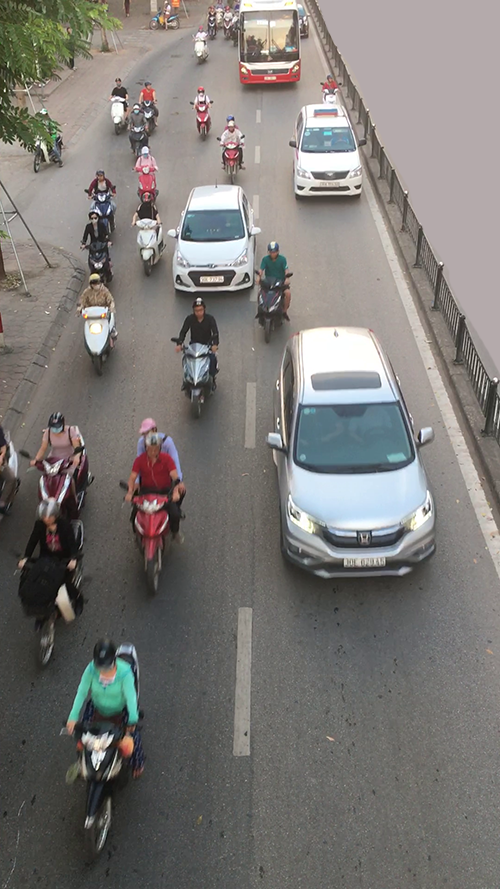
\includegraphics[width=0.7\textwidth]{Chapters/Fig/09}
      \caption{Image 1}
      \label{fig:img09}
  \end{figure}
\end{center}

\begin{center}
    \begin{figure}[H]
        \centering
      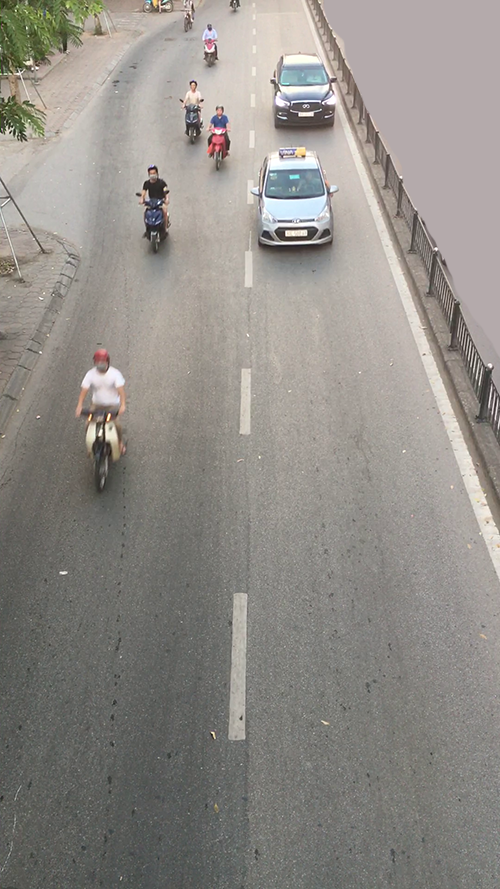
\includegraphics[width=0.7\textwidth]{Chapters/Fig/10}
      \caption{Image 10}
      \label{fig:img10}
  \end{figure}
\end{center}

\begin{center}
    \begin{figure}[H]
        \centering
      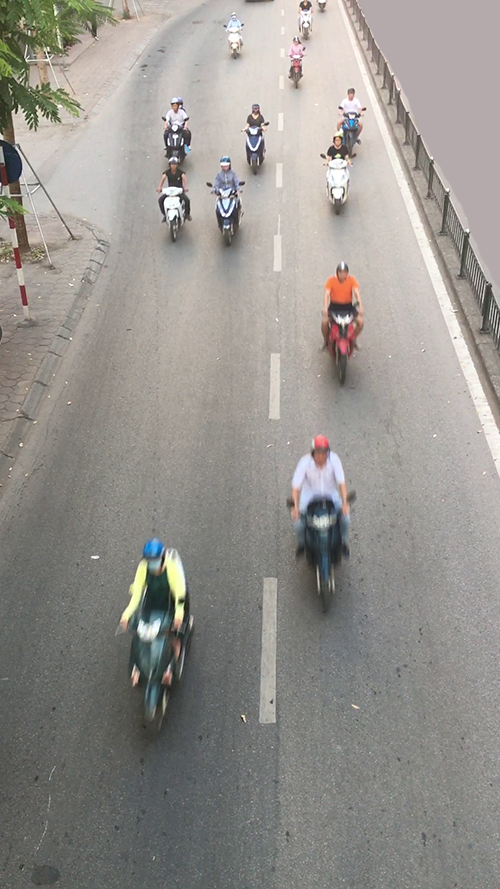
\includegraphics[width=0.7\textwidth]{Chapters/Fig/11}
      \caption{Image 11}
      \label{fig:img11}
  \end{figure}
\end{center}

\begin{center}
    \begin{figure}[H]
        \centering
      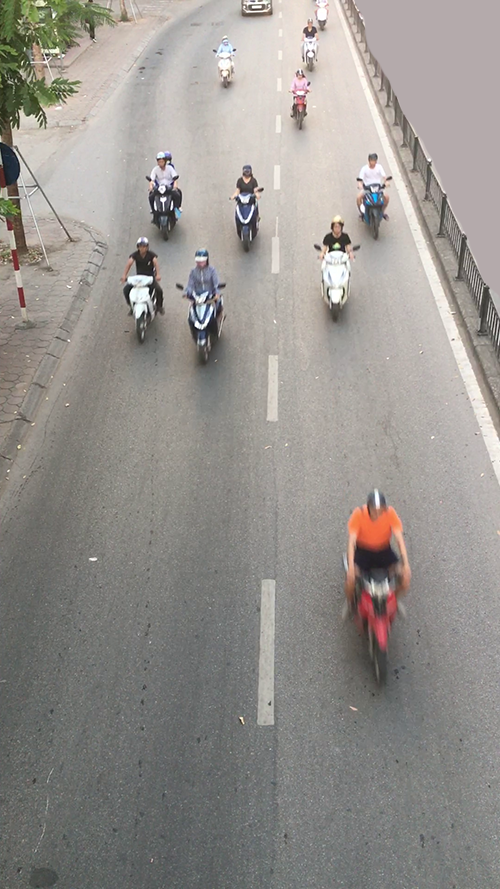
\includegraphics[width=0.7\textwidth]{Chapters/Fig/12}
      \caption{Image 12}
      \label{fig:img12}
  \end{figure}
\end{center}

\begin{center}
    \begin{figure}[H]
        \centering
      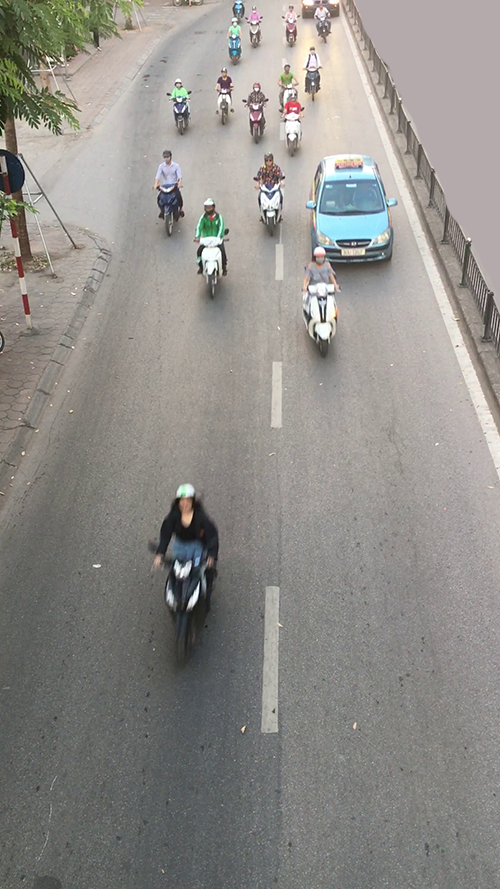
\includegraphics[width=0.7\textwidth]{Chapters/Fig/13}
      \caption{Image 13}
      \label{fig:img13}
  \end{figure}
\end{center}

\begin{center}
    \begin{figure}[H]
        \centering
      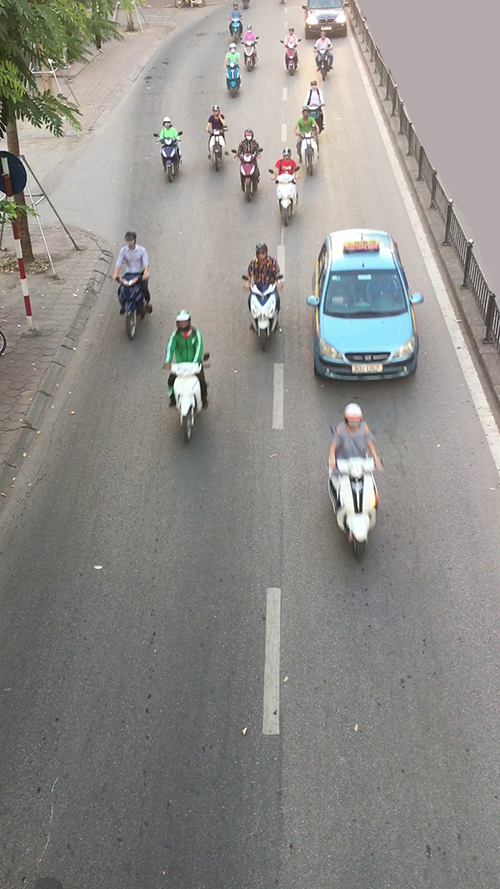
\includegraphics[width=0.7\textwidth]{Chapters/Fig/14}
      \caption{Image 14}
      \label{fig:img14}
  \end{figure}
\end{center}

\begin{center}
    \begin{figure}[H]
        \centering
      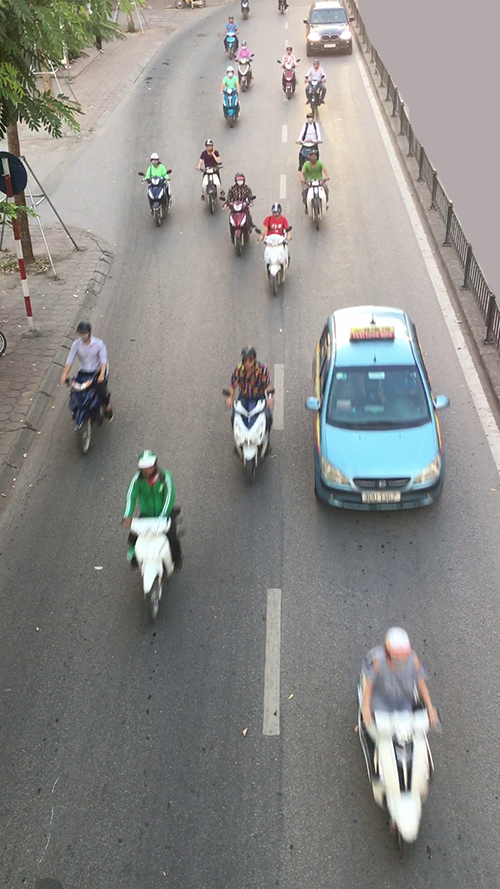
\includegraphics[width=0.7\textwidth]{Chapters/Fig/15}
      \caption{Image 15}
      \label{fig:img15}
  \end{figure}
\end{center}